Machine learning (ML) is an increasingly popular data analytic technique widely employed not limited to particle physics. It is useful for scenarios where a large amount of data generated or observed requires analyses that cannot simply be done by traditional statistical techniques. In high energy physics, the use of machine learning has made a significant impact especially in the discovery of the Higgs boson using Boosted Decision Trees \cite{chatrchyan2012observation, aad2012observation, chen2015higgs}. However, machine learning is not an all-mighty tool that could discover new physics. Applying existing conditions to searches reduces unwanted information, resulting in the algorithm working harder but allowing it to optimize its search for new physics. This process is known as \textit{pre-selection}, and it is a crucial step in our method. \\


%-------------------------------------------------------------------------%
\section{Machine learning}
Machine learning is an umbrella term for algorithms that ``learns" patterns from a given data set whether small or large to give predictions. There are two general categories in ML, which are known as \textit{supervised learning} and \textit{unsupervised learning}. Supervised learning requires a separate data with labeled outcomes (simulations) to build an effective model for analyzing the raw data whose outcomes are not labeled. This process is known as \textit{training}. Unsupervised techniques, on the other hand, do not require training as they are purely data-driven methods opposed to relying on simulations like supervised techniques. Unbalanced and difficult datasets produced in collider experiments are most effective with supervised techniques, and so ML referred to hereon will imply supervised techniques. \\

Training a dataset is relatively simple. The process involves importing the data onto the chosen platform, choosing which algorithm to use and follow its syntax in building a model, including which parameters to use. Most existing open-source algorithms are extremely versatile and already yield a high performance, which allows for easy use. Models are built by minimizing a chosen error, where common choises are simple metrics such as \textit{Mean Squared Error (MSE)}, \textit{Residual MSE (RMSE)}, \textit{Log-loss} etc. However, when training a classifier one must be careful of \textit{overtraining}, a relatively common error that many encounter. Overtraining occurs when a model's parameters are too restrictive, limiting a model to be versatile in its performance. Versitility here implies that how a model performs under various datasets that are similar in nature. In other words, by restricting a model to perform well under a single dataset, we limit ourselves in performing well when it counts i.e. the raw data. \\

Overtraining is not a difficult mistake to avoid. Cross-validations (CV) is an effective method to prevent overtraining. CV is a task that requires the training data to be further partitioned to create a smaller set of training and test data. The most common CV is the \textit{k-fold CV}, where the training data is randomly sampled into $k$ different subsets. By selecting $k-1$ of these subsets as the training data to build the classifier on, the remaining subset is used to validate this model on. This procedure is repeated $k$ times through each split, where each performance is scored. The overall result typically involves taking the average of the $k$-fold scores.  There are no set rules on what the best value of $k$ is, however, most ML users prefer to stick to either 5 or 10 due to its simplicity and performance yield \cite{james2013introduction}. \\

Upon building a classifier, it is difficult to find the most optimal parameters whilst being cautious of overtraining. In order to overcome this dilemma, a grid search can be performed. A grid search utilizes CV at its foundations to test the performance of the selected parameters. By utilizing this feature, it is possible to check through a range of parameters. The down-side to this, however, is that it is computationally expensive and multiple evaluations may be required to even find some consistency in the results before narrowing down some parameters. \\

Fine-tuning parameters is not the only effective method to improve the classifier. A common technique known as \textit{feature engineering} can be employed to manipulate the existing variables so that the prediction accuracy improves across the models built, although not guaranteed. In this work, a simple feature engineering was performed. This entailed of rearranging the four jet entries such that the highest $p_T$ jet with a b-tag is considered the b-jet originating from the decay, and the subsequent jets are ordered by the $p_T$ values regardless of whether there is a b-tag or not. \\

The most popular algorithms employed by the scientific community (not limited to physics) are Neural Networks (NNs) and Decision Trees (DTs). In the correct setting, either methods perform exceptionally well. The trend in many communities favour NNs over DTs. However, through some preliminary tests using the \textit{h2o} package's \textit{automl} function, it was shown that a tree-based method known as \textit{Extreme Gradient Boosting (EGB)} is most suited for this task. The package that contains this feature is known as \textit{xgboost}, both available as a standalone use or an extension of the h2o package. \\

%-------------------------------------------------------------------------%
\section{Tree-based methods and Extreme Gradient Boosting}

Tree-based methods can intuitively be thought of as an extension to a cut-flow analysis. Instead of discarding selections that do not fulfill a certain criteria, these selections may be further explored upon by the algorithm provided that a new criteria exists. A simple diagram is depicted in Figure \ref{fig:tree}, where the mathematical form of it is described in Equation \ref{eq:DT}. Here, $c_m$ is the ..............

\begin{figure}[htbp]
    \centering
    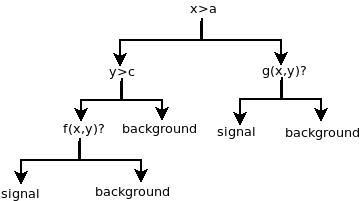
\includegraphics[width=10cm, height= 6cm]{DT.png}
    \caption{A simple decision tree for a hypothetical signal selection, expanding on Figure \ref{fig:cut} such that an extra parameter $g(x,y)$ is present within the algorithm.}
    \label{fig:tree}
\end{figure}

\begin{equation}
    f(x) = \sum_{i=1}^m c_m I(x\in R_m)
    \label{eq:DT}
\end{equation}

There are many tree-based methods such as random forests, where the method of sampling the data and how a loss-function is minimized. In the case of EGB models, WRITE MORE ABOUT XGBOOST \\

The performance of a classifier can be boiled down a single table known as a confusion matrix. Displayed in Table \ref{tab:ConfMat}, a confusion matrix visually shows the distribution of correctly and incorrectly classified points within the dataset. The correctly classified signal and background events are the True Positives (TP) and True Negatives (TN), respectively. Likewise, the incorrectly classified signal and background events are the False Negatives (FN) and False Positive (FP), respectively. The accuracy of the classifier is given by TP+TN/N, and the higher the accuracy, the higher the SBR. \\

% Confusion matrix template
\begin{table}[htbp]
    \centering 
    \begin{tabu}{c|[2pt]c|c|c|c}
        \multicolumn{2}{c}{}&\multicolumn{2}{c}{Predicted}&\\
        \tabucline[2pt]{3-5}
        \multicolumn{2}{c|[2pt]}{}
        &\multicolumn{1}{c|}{Background} &\multicolumn{1}{c|[2pt]}{Signal} &\multicolumn{1}{c|[2pt]}{Total}\\
        \tabucline[2pt]{2-5}
        \multirow{\items}{*}{\rotatebox{90}{Simulated}}
        &\multicolumn{1}{c|[2pt]}{Background} & \multicolumn{1}{c|}{TN} & \multicolumn{1}{c|[2pt]}{FP} & \multicolumn{1}{c|[2pt]}{TN$+$FP} \\
        \cline{2-5}
        \multicolumn{1}{c|[2pt]}{}& \multicolumn{1}{c|[2pt]}{Signal} & \multicolumn{1}{c|}{FN} & \multicolumn{1}{c|[2pt]}{TP} & \multicolumn{1}{c|[2pt]}{FN$+$TP} \\
        \tabucline[2pt]{2-5}
        \multicolumn{1}{c|[2pt]}{} & \multicolumn{1}{c|[2pt]}{Total} & \multicolumn{1}{c|}{TN$+$FN} & \multicolumn{1}{c|[2pt]}{FP$+$TP} & \multicolumn{1}{c|[2pt]}{N}\\
        \tabucline[2pt]{2-5}
    \end{tabu}
    \caption{A confusion matrix for truth (simulated) and predicted labels and its components.}
    \label{tab:ConfMat}
\end{table}

An evaluation metric presented by the Higgs Challenge \cite{adam-bourdarios_learning_2014} is the \textit{approximate median significance (AMS)}, given by the equation
\begin{equation}
    \text{AMS} = \sqrt{2\Big((s+b+b_r)\ln\Big(1+\frac{s}{b+b_r}\Big)\Big)}
    \label{eq:AMS}
\end{equation}
where $s$ and $b$ are the unnormalized TP and FP rates, respectively, and $b_r$ is a constant regularization term set at 10.
%-------------------------------------------------------------------------%
%\section{}


%-------------------------------------------------------------------------%